Vor allem wegen seiner Effizienz und Genauigkeit hat sich  in einer Vielzahl
von Anwendungen bewährt:
\begin{itemize}
    \item \textbf{Bilderkennung und Computervision:} Gesichtserkennung~\cite{viola2001rapid}
          \begin{figure*}
              \centering
              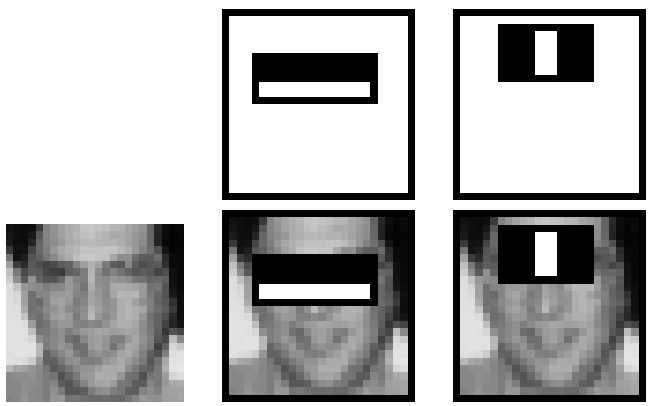
\includegraphics[width=.65\textwidth]{figures/CV_Example.png}
              \caption{Anwendung von AdaBoost bei Computer Vision:
                  Features messen Kontraste in bestimmten Gesichtsregionen\cite{viola2001rapid}}
          \end{figure*}
    \item \textbf{Textklassifikation und Natural Language Processing}: Erkennung von Spam-Mail~\cite{panwar2022detection}
          \begin{figure*}
              \centering
              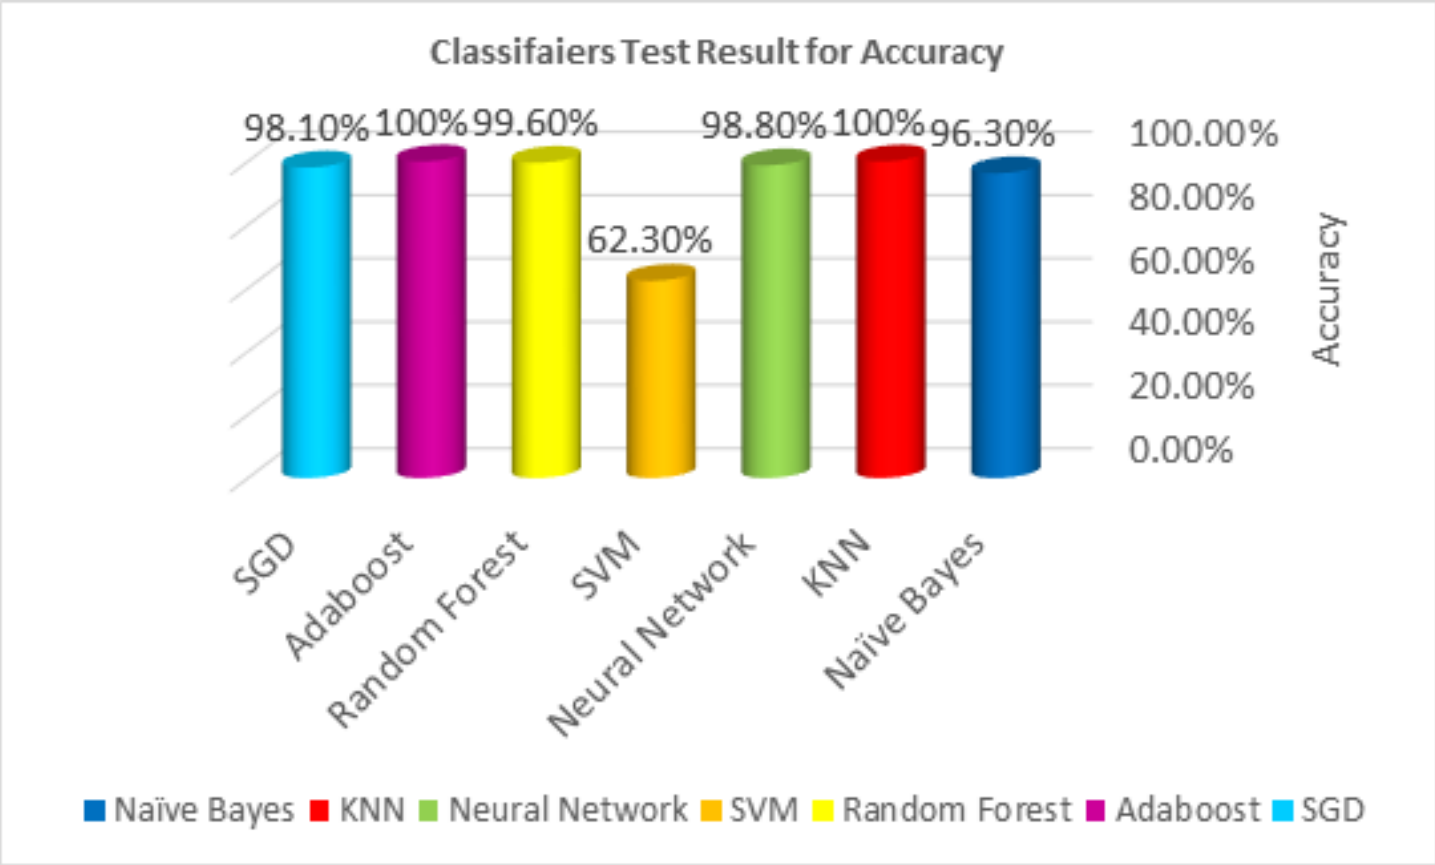
\includegraphics[width=.65\textwidth]{figures/spam.png}
              \caption{Erkennung von Spam-Mail durch AdaBoost im Vergleich zu anderen Verfahren\cite{panwar2022detection}}
          \end{figure*}
    \item \textbf{Medizinische Diagnostik:} Risiko/Erkennung von Krankheiten baserend auf Patientendaten~\cite{hatwell2020ada}
          \begin{figure*}
              \centering
              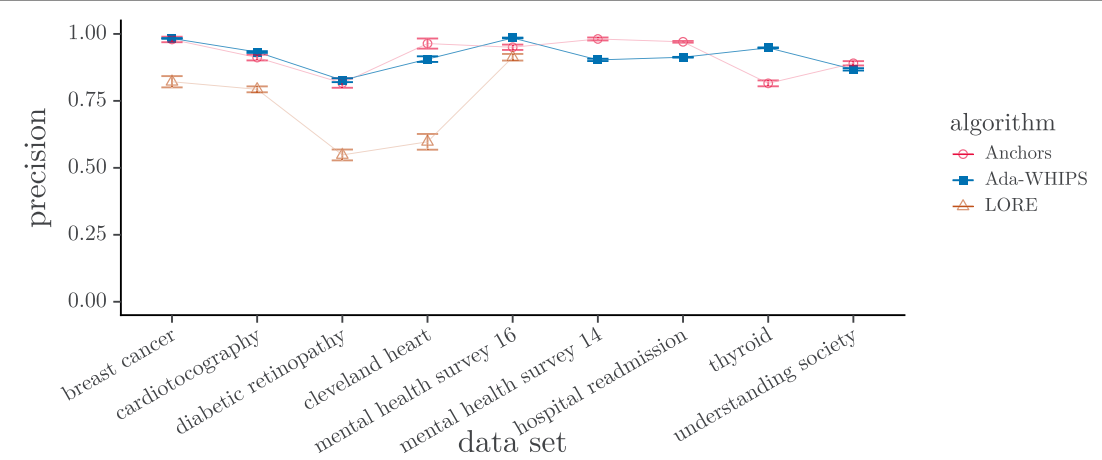
\includegraphics[width=.65\textwidth]{figures/ada-whips.png}
              \caption{Diagnostik mit AdaBoost im Vergleich \cite{hatwell2020ada}}
          \end{figure*}
    \item \textbf{Finanzwesen:} Vorhersage von Aktienkursbewegungen~\cite{zhang2016stock}
          \begin{figure*}
              \centering
              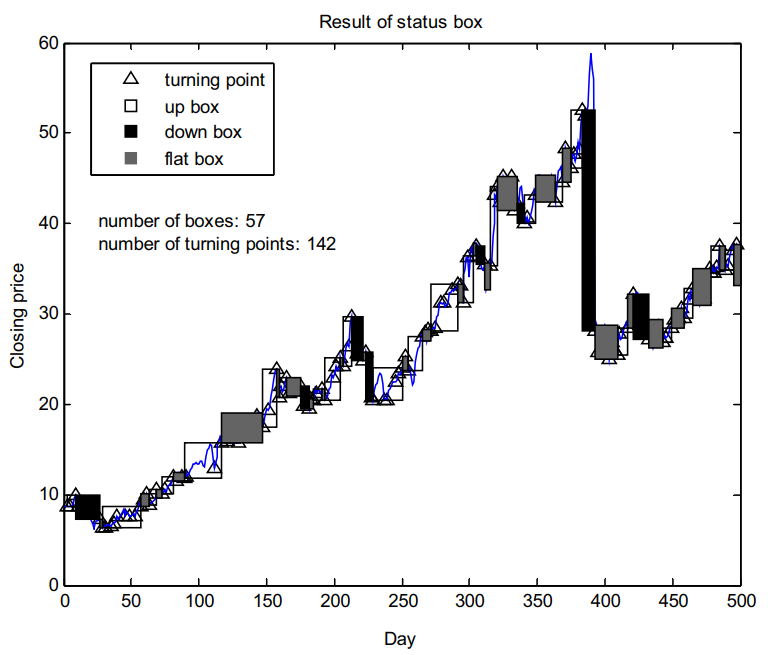
\includegraphics[width=.65\textwidth]{figures/stock.png}
              \caption{Vorhersage von Kursbewegungen mit AdaBoost. Boxen fassen Schlusspreise als Features zusammen. \cite{zhang2016stock}}
          \end{figure*}
\end{itemize}



